% !TEX root = 99_main.tex

An experient was conducted at co-working spaces at the National Unviersity of Singapore. 15 participants were recruited for the experiment and equiped with a fitbit watch. The watch settings were set to also request thermal preference (prefer warmer, prefer cooler, comfy), and the set to force request feedback at the hours of 9:00, 11:00, 13:00, 15:00, and 17:00. 

The watch was further complimented with IoT connected on-body and environmental sensors. The onbody sensor consists of a temperature and light sensor from mbient-labs that had been modified to fit the watch strap with a custom 3d printed case. An off body sensor measuring temperature and humidity was attached to the participants bag. The sensors communicate via bluetooth to raspberryPi gateways that had been positioned throughout the working space. 

Data from the cozie watch face, and the environmental sensors were aggrigated in an Influx cloud time-series database, which served as a platform for data aquisition and fault detection. Source codes can be found here \cite{aurek-data}.


% \begin{figure}
% \begin{center}
% 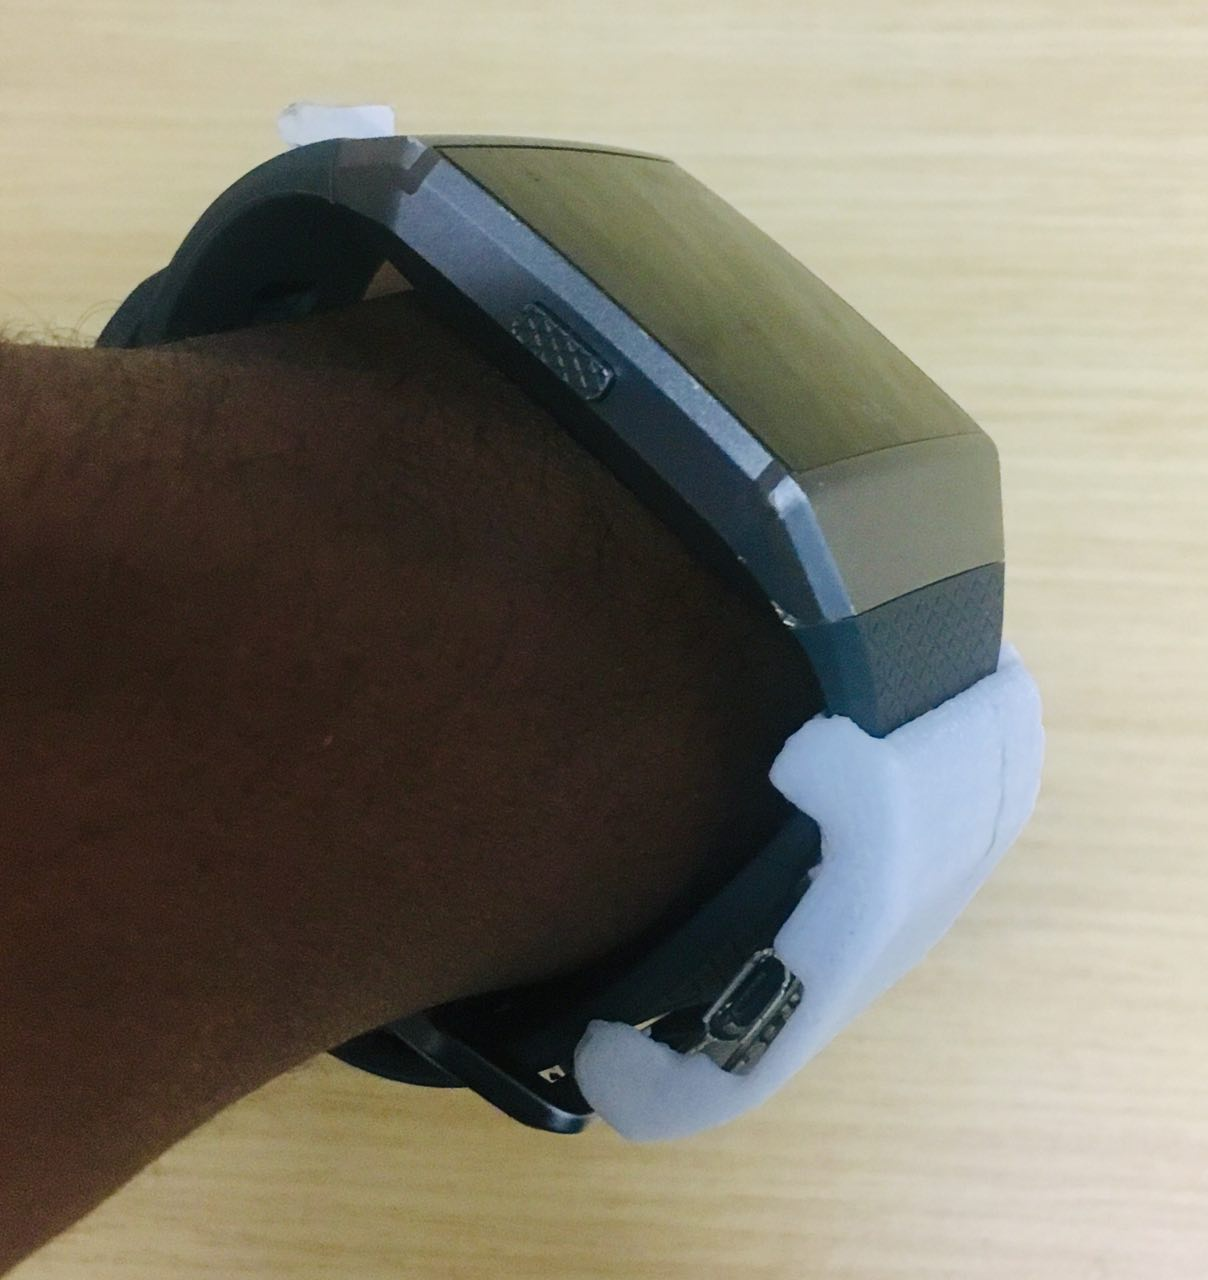
\includegraphics[width=0.2\textwidth, trim= 0cm 0cm 0cm 0cm,clip]{strap-pack.jpg}
% \caption{Strap-Pack}
% \label{fig:strappack}
% \end{center}
% \end{figure}

